\begin{figure*}[t]
\centering
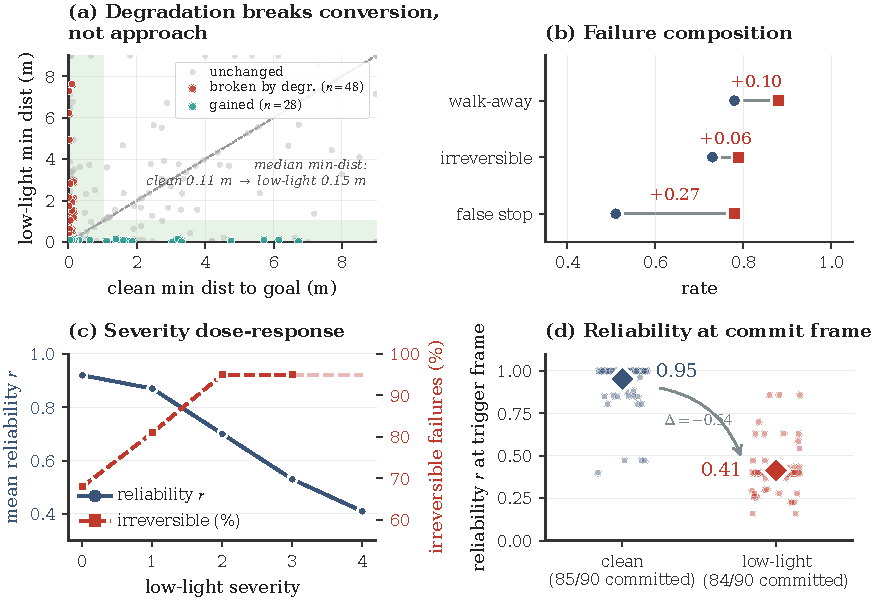
\includegraphics[width=\textwidth]{figures/fig_motivation.pdf}
\caption{\textbf{Method-independent motivation study (baseline InstructNav).}
\textbf{(a)}~Per-episode paired minimum distance to goal on the \emph{same}
$300$ episodes run clean and under low-light~s4: the approach geometry
barely moves (median min-dist $0.11\to0.15$\,m) yet $48$ episodes flip to
failure (red)---degradation breaks the reach-to-success \emph{conversion},
not the approach.
\textbf{(b)}~M2 ($n{=}90$): degradation shifts failures toward walk-aways and
irreversible failures, and false stops nearly double (walk-away and
irreversible: fraction of failed episodes; false stop: fraction of executed
stops that are false positives).
\textbf{(c)}~M3: as severity rises, mean reliability falls and the irreversible
fraction saturates at $95\%$.
\textbf{(d)}~M4: the deciding commitment fires on a single low-$r$ frame (mean
$r$ drops $0.95{\to}0.41$); once committed the agent stays locked for
${\sim}21$ steps. Coloured dots in (d) jitter the underlying per-commit $r$
distribution; diamonds are the means. $N$ counts episodes in which a commit
fired ($85$ and $84$ of the $90$ per condition; the remainder never
committed).}
\label{fig:motivation}
\end{figure*}

\section{Why Navigation Fails Under Degradation}
\label{sec:motivation}

A single episode previews the phenomenon this section quantifies. Asked to
find a toilet under low light, the baseline agent navigates to within
$0.02$\,m of it, never declares it found, wanders off, and the episode ends
in failure (Figure~\ref{fig:case-studies}c). The agent saw enough to get
there; what failed was the decision to stop. This section shows that the
pattern is systematic.

We analyze how visual degradation causes a zero-shot
navigator to fail. Every quantity is measured on the unmodified backbone, so
that the analysis does not depend on any component of our method. We organize
the study as five questions (M0--M4): whether degradation hurts at all (M0),
whether the cause is appearance (M1), what failures look like (M2), whether
reliability is informative about commitments (M3), and what triggers a
commitment (M4).

\paragraph{Setup.}
We run InstructNav on HM3D ObjectNav \texttt{val\_mini} pooled over seeds
$\{0,1,2\}$ ($n{=}90$, bootstrap $95\%$ CIs, $B{=}5000$). The primary
degradation is low-light at severity~$4$, drawn from a $13$-type
ImageNet-C-style suite \citep{hendrycks2019benchmarking}. The $n{=}90$
study below establishes the qualitative chain; the Experiments section
re-measures decisive quantities at $N{=}300$.

\paragraph{M0--M1: Degradation hurts, but appearance is not the lever.}
Low-light lowers SR from $0.433$ (CI $[0.333, 0.533]$) to $0.222$ ($[0.144,
0.311]$) at $n{=}90$; the paired drop is $-0.211$ with CI $[-0.322, -0.100]$,
excluding zero. Motion-blur gives $-0.056$ with CI
$[-0.167, +0.056]$ and does not exclude zero, so we use low-light as the
primary condition. Figure~\ref{fig:motivation}a shows \emph{where} the drop
lives at the paired $N{=}300$ scale: the per-episode minimum distance to
the goal is nearly unchanged (median $0.11\to0.15$\,m)---the agent still
gets to the goal---yet $48$ episodes flip to failure. Adding a test-time
restoration arm raises PSNR on
low-light from $7.4$ to $15.9$\,dB ($+8.4$\,dB) yet SR moves only $0.233
\to 0.300$, inside the $\pm0.10$ seed-noise band: making the image look
clean does not make the agent navigate.

\paragraph{M2: Failures are irreversible commitments.}
To characterize the failures, we distinguish \emph{walk-away} failures (the
agent ends far from a reachable goal and never returns) from \emph{false
stops} (premature, false-positive stops). A walk-away
is \emph{irreversible} when the trajectory was once closer to the goal but then
moved away and never came back. Degradation shifts the composition of failures
toward walk-aways: among failed episodes, the walk-away fraction rises from
$78\%$ on clean input to $88\%$ under low-light, and the irreversible fraction
from $73\%$ to $79\%$ (Figure~\ref{fig:motivation}b). The false-stop rate---the
fraction of executed stops that are false positives---rises in parallel, from
$0.51$ to $0.78$. Moreover, the reliability at the turning point $t^\star$,
where $d_t$ switches from decreasing to increasing, drops from $0.93$ on clean
input to $0.40$. The failures are thus not a matter of insufficient
exploration; they are early, confident commitments made when perception is
untrustworthy.

\paragraph{M3--M4: Reliability is informative; a single low-$r$ frame triggers the commitment.}
The reliability estimate carries a usable signal. On clean input, bucketing
commitments by $r$ shows net geodesic progress over the next five steps
rising monotonically with $r$ ($0.133/0.154/0.245$ for low/mid/high), and
across severities $0$--$4$ the mean $r$ falls monotonically
($0.92{\to}0.87{\to}0.70{\to}0.53{\to}0.41$) while the irreversible
fraction saturates at $95\%$ by severity~$3$ (Figure~\ref{fig:motivation}c).
The commitment itself is a single-frame event: the detector's
\texttt{found} flag flips on one frame, not after temporal consensus.
Across conditions, the $r$ of that triggering frame falls from $0.95$ on
clean to $0.41$ under low-light ($85$ and $84$ of the $90$ episodes per
condition committed at least once), and once made the
commitment persists for ${\sim}21$ steps (Figure~\ref{fig:motivation}d).
The entry point of the failure is an irreversible decision on one
unreliable frame.

\paragraph{M5: A reachability/commit-loss decomposition at the $N{=}300$ scale.}
The $M$-study above uses $n{=}90$; we now confirm the mechanism at the
$N{=}300$ main-split scale, where the baseline success rate is $0.36$ rather
than the $0.22$ of \texttt{val\_mini}. We decompose the outcome as
$\text{SR} = \text{reachability} - \text{commit/stop loss}$, where reachability
is the fraction of episodes whose trajectory passes within $1.0$\,m of the goal
(an upper bound achievable by a perfect stop policy on the \emph{actual}
trajectory, requiring no re-run; the threshold is calibrated from the $p_{90}$
stopping distance of clean successes, $0.15$\,m). On low-light at severity~$4$,
the baseline reaches within $1.0$\,m in $62.3\%$ of episodes but succeeds in
only $35.8\%$, a commit/stop loss of $26.5$ points: in one episode out of four
the agent passes the goal and fails to convert. Crucially, degradation does not
suppress \emph{action}: the commit rate is $93\%$ under low-light versus $94\%$
on clean input, and the pure-exploration-failure rate is ${\sim}6\%$ at both
ends. What collapses is commitment \emph{quality}: the reliability at the
committing frame falls from $0.95$ to $0.39$, the false-commit rate rises from
$55\%$ to $76\%$, only $40\%$ of commitments lead to success, and the agent
stays locked for ${\sim}12$ steps (${\sim}21$ in the $n{=}90$ study; the lock
is shorter on the easier main split but present at both scales). The same decomposition holds for
Gaussian noise (reachability ${\sim}0.59$, the loss again dominant), so the
pattern is not specific to low light.

\paragraph{Summary.}
The observations form a consistent chain: degradation does not blind the
agent and does not stop it from acting; it leads the agent to stake
irreversible heading and stop commitments on single, low-reliability
frames, so the resulting loss sits in the reach-to-success conversion
rather than in perception or exploration. The diagnosis predicts that
interventions on appearance or on where-to-go should not move success,
because they never touch the commitment conversion. The Method section
turns this into candidate interventions; the Experiments section confirms
the prediction across a six-family sweep in which no deployable arm moves
success and several lower it.
